\section{Ziel}
\label{sec:Ziel}
Es wird die Wechselwirkung energiereicher Strahlung mit Materie untersucht.
Hierzu wird die Reichweite von $\beta^-$-Strahlung in Materie, etwa bei Transmission durch dünne Blenden, betrachtet sowie der Wirkungsquerschnitt $\sigma$ und Absorptionskoeffizient $\mu$ verschiedener Materialien bei $\gamma$-Strahlung ermittelt.

\section{Theorie}
\label{sec:Theorie}

\subsection{Wirkungsquerschnitt \texorpdfstring{$\sigma$}{Sigma} und das Absorptionsgesetz}
\label{sec:absorp}
Die $\gamma$-Strahlung ist Photonen-Strahlung, $\beta^-$-Stahlung ist Materie-Strahlung von energiereichen Elektronen.
Beide Strahlungsarten treten beim Propagieren in Wechselwirkung mit Materie, wodurch sie absorbiert werden können.
% im Bereich von \SI{60}{\kilo}eV bis \SI{1300}{\kilo}eV.
%Für die $\gamma$-Strahlung wird ein Absorptionsgesetz beschrieben.
%Beim Eindringen in die Materie treten die Photonen mit den Atomen in Wechselwirkung. 
%je tiefer eingedrungen wird, desto wahrscheinlicher ist dieWechselwirkung.
%Dadurch nimmt die Anzahl der Photonen pro Zeit und Fläche ab; mit der Eindringtiefe nimmt die Wahrscheinlichkeit zu, 
%dass das Photon gestoßen hat.

Als Maß für die Häufigkeit dieser Wechselwirkung wird der Wirkungsquerschnitt $\sigma$ eingeführt.
$\sigma$ ist eine Fläche bestimmter Größe, die dem Absorber spezifisch zugeordnet wird. 
Dabei wird angenommen, dass der Absorber punktuell aus diesen Flächen $\sigma$ besteht und nur an diesen Stellen zum Aufhalten der Strahlung in der Lage ist.
Trifft in diesem Modell ein Photon oder ein Elektron auf eine dieser Flächen, wird es absorbiert; andernfalls durchdringt die Strahlung die Materie unbeeinflusst.
Es wird die Wahrscheinlichkeit $W$ beschrieben, mit welcher ein eintreffendes Strahlungsteilchen auf eine dieser Flächen trifft. 
Dabei gilt die Beziehung 
\begin{equation}
	W=n D \sigma =\frac{n D \sigma F}{F},
\end{equation}
in welcher im Weiteren $D$ die Schichtdicke des Absorbers und $F$ die Querschnittsfläche ist. 
$n$ beschreibt die Anzahl der Absorber-Teilchen pro Volumeneinheit.
Treffen $N_0$ Teilchen in einem Zeitintervall auf die Fläche $F$, kann über
\begin{equation}
	N=N_0 n D \sigma
\end{equation}
die Anzahl $N$ der Wechselwirkungen im gewählten Zeitintervall bestimmt werden. 
In einem realen Absorber überdecken sich die $n$ Volumeneinheiten teilweise. 
Dies hat zur Folge, dass die ungewollte Überdeckung nur vernachlässigbar ist, wenn eine dünne Schicht mit der Dicke $\mathup{d}x$ betrachtet wird, in der $\mathup{d}N$ Reaktionen stattfinden. 
Damit ist
\begin{equation}
	\mathup{d}N=-N(x)  n \sigma \mathup{d}x.
	\label{eq:Absorptionsgesetz_Vorstufe}
\end{equation}

Die Anzahl der Strahlungsteilchen, die erst nach der Strecke $\mathup{d}x$ mit der Materie wechselwirken, nimmt um $N(x)$ ab. 
Wird Gleichung \eqref{eq:Absorptionsgesetz_Vorstufe} über die Dicke $D$ des Absorbers integriert, ergibt sich das Absorptionsgesetz
\begin{equation}
	N(D)=N_0 \exp(-n \sigma D)=N_0 \exp(-\mu D),
	\label{eq:Absorptionsgesetz}
\end{equation}
in welchem der Absorptionskoeffizient $\mu=n\sigma$ eingeführt wird.
Dieses exponentielle Absorptionsgesetz gilt unter der Annahme, dass die Teilchen der Strahlung nur einmal mit dem Material stößt und dabei vollständig abgebremst und absorbiert werden.
Nach der spezifischen Größe
\begin{equation}
	D_{\sfrac{1}{2}}=\frac{\ln(2)}{\mu},
\end{equation}
ist eine Absorberdicke gefunden, bei welcher sich die Intensität der Strahlung im Schnitt halbiert hat.
Die Anzahl $n$ der Stoßpartner im Absorber pro Volumeneinheit wird mit
\begin{equation}
	n=\frac{zN_\text{L}}{V_\text{Mol}}=\frac{zN_\text{L}\rho}{M}
\end{equation}
abgeschätzt, wodurch 
\begin{equation}
%\sigma_C=2\pi  r_e²\left(\frac{1+\epsilon}{\epsilon²}\left(\frac{2(1+\epsilon)}{1+2\epsilon}-\frac{1}{\epsilon}\ln(1+2\epsilon)\right)+\frac{1}{2\epsilon}\ln(1+2\epsilon)-\frac{1+3\epsilon}{(1+2\epsilon)²}\right)
	\sigma=\frac{M\mu}{zN_\text{L}\rho}
	\label{eq:Wirkungsquerschnitt}
\end{equation}
gilt.
In Gleichung \ref{eq:Wirkungsquerschnitt} sind $z$ die Ordnungszahl des Absorberatoms, $N_\text{L}$ die Loschmidtsche Zahl, $V_\text{Mol}$ das Molvolumen, $M$ das Molekulargewicht und $\rho$ Dichte.

\subsection{\texorpdfstring{$\gamma$}{Gamma}-Strahlung und ihre Wechselwirkungsprozesse mit Materie}
\label{sec:gamma}
Wenn ein angeregter Atomkern in einen energetisch günstigen Zustand zurückfällt, wird die frei werdene Energie in Form von $\gamma$-Strahlung emittiert. 
$\gamma$-Strahlung ist eine elektromagnetische Welle, welcher eine Wellenlänge zugeordnet werden kann. 
Es gilt hierzu
\begin{equation}
	E =h\frac{c}{\lambda}.
\end{equation}
Die Energieniveaus der Kerne sind sehr genau definiert, daher besitzt das Linienspektrum diskret und präzise bestimmbar.
Für die Energiewerte, die für die verwendete, natürliche Strahlungsquelle angenommen werden, treten im Wesentlichen drei Prozesse auf.
Die hier auftretenden Vertreter der Prozesse werden im Folgenden diskutiert.

\begin{itemize}
\item{\emph{(innerer) Photoeffekt}}

Trifft das $\gamma$-Quant auf ein Elektron, überträgt es beim Photoeffekt die gesamte Energie auf dieses und verschwindet. 
Das gestoßene Elektron wird aus seiner Bindung im Atom herausgelöst und besitzt die kinetische Energie $E_e=h\nu-E_\text{B}$ mit der zu überwindenden Elektronen-Bindungsenergie $E_\text{B}$. 
Der Photoeffekt kann nur ablaufen, wenn die Energie der Strahlung größer als die Bindungsenergie des Elektrons $E_\text{B}$ ist. 
Außerdem tritt er nur ein, wenn das Atom den Quantenimpuls des $\gamma$-Quantes aufnehmen kann. 
Dies ist umso wahrscheinlicher, je fester das Elektron an das Atom gebunden ist und tritt deswegen bei typischen $\gamma$-Energien nur bei inneren Elektronen auf. 
Die entstehenden Lücken werden durch äußere Elektronen unter Emission von Röntgenstrahlung und Auger-Elektronen aufgefüllt.
\item{\emph{Compton-Effekt}}

Das $\gamma$-Photon wird im Zuge des Compton-Effekts an einem freien Elektron oder an einem Elektron in der äußeren Hülle gestreut und gibt seine Energie zum Teil an dieses ab. 
Dies ruft eine Richtungs- und Impulsänderung hervor, erhält aber das $\gamma$-Photon.
Der Wirkungsquerschnitt $\sigma_\text{C}$ wird durch
\begin{equation}
	\sigma_\text{C}=2\pi  r_e^2\left(\frac{1+\epsilon}{\epsilon²}\left(\frac{2(1+\epsilon)}{1+2\epsilon}-\frac{1}{\epsilon}\ln(1+2\epsilon)\right)+\frac{1}{2\epsilon}\ln(1+2\epsilon)-\frac{1+3\epsilon}{(1+2\epsilon)²}\right)
\label{eq:sigma_c}
\end{equation}
mit $\epsilon=\frac{E_{\gamma}}{m_0c²}$ und dem kleinsten Elektronenradius $r_e=\SI{2.82e-15}{\meter}$ beschrieben. 
Damit ergibt sich
\begin{equation}
	\mu_\text{C}=n\sigma_\text{C}(\epsilon)=\frac{Z N_L \rho}{M}\sigma_\text{C}(\epsilon).
\label{eq:mu_c}
\end{equation}
\item{\emph{Paarerzeugung}}

Ist die Energie des $\gamma$-Quants sehr groß, kann es unter Erzeugung von Elektron und Positron zur Paarbildung kommen.
Es ist einerseits erforderlich, dass das $\gamma$-Quant eine Energie $E$ größer als die doppelte Ruheenergie eines Elektrons, und andererseits, dass ein Teil des Impulses von einem weiteren Stoßpartner übernommen wird.
Hierzu dienen die Atomkerne des Absorbermaterials, in  deren Coulomb-Feldern  sich die  Teilchenpaare bilden.
\end{itemize}
\begin{figure}
	\centering
	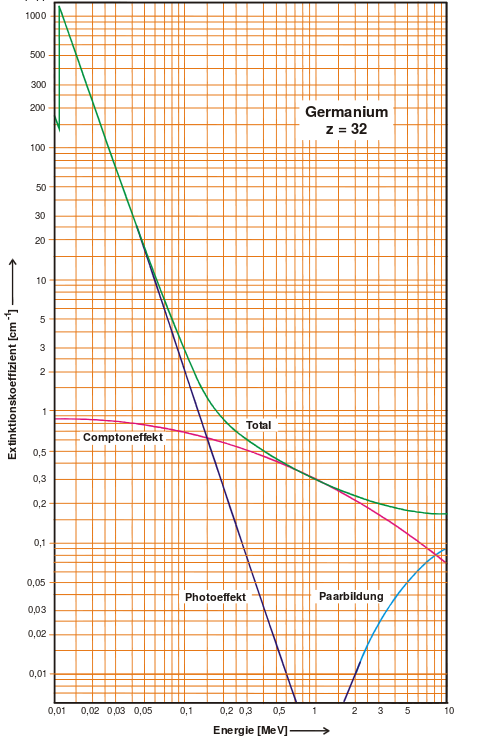
\includegraphics[width=0.5\textwidth]{Bilder/germanium.png}
	\caption{Eintrittswahrscheinlichkeit der verschiedenen Wechselwirkungsprozesse von \texorpdfstring{$\gamma$}{Gamma}-Strahlung mit Germanium.\cite{skript}}
	\label{fig:Germanium}
\end{figure}
Die Überlagerung der oben genannten Effekte ergibt die Totalkurve, die als Beispiel von Germanium in Abbildung \ref{fig:Germanium} gezeigt wird.
Weiter kann dieser Abbildung entnommen werden, bei welcher Energie die Effekte dominant sind.
In Reihenfolge treten bei ansteigender Energie Photoeffekt, Compton-Effekt und Paarerzeugung auf.


\subsection{\texorpdfstring{$\beta^-$}{Beta}-Strahlung und ihre Wechselwirkungsprozesse in Materie}
\label{sec:beta}

$\beta^-$-Strahlung entsteht bei dem Zerfall von Nukleonen.
Bei dem Zerfall eines Protons zu einem Neutron wird ein $\beta^-$-Teilchen -- ein energiereiches Elektron -- und ein Anti-Neutrino emittiert.
Diese Kombination garantiert die Erhaltung von Energie, Impuls und Drehimpuls.
Das Neutrino hat halbzahligen Spin, trägt keine Ladung und tritt (unter anderem daher) mit Materie nicht in Wechselwirkung.
Die frei werdende Energie verteilt sich auf die emittierten Teilchen und dem rückgestoßenen Kern.
Dies ist in Abbildung \ref{fig:energieElektron} dargestellt.

Anders als bei $\gamma$-Strahlung im vorangegangen Abschnitt wird für  $\beta^-$-Strahlung kein geschlossenes Absorptionsgesetz in vergleichbarer Kürze beschrieben.
Die $\beta^-$-Strahlung tritt über verschiedene Prozesse mit Materie in Wechselwirkung, die wesentlichen Effekte werden im Folgenden diskutiert.

\begin{itemize}
	\item{\emph{Elastische Streuung am Atomkern:}}

Die elastische Streuung an dem Atomkern ist als Rutherford-Streuung bekannt.
Es handelt sich um eine Streuung der $\beta^-$-Strahlung im Coulomb-Feld der Kerne, wodurch der eintreffende Strahl wesentlich abgelenkt und dadurch aufgefächert, allerdings nicht besonders abgebremst wird.
Durch mehrfache Ablenkung ist die Länge der Bahn eines $\beta^-$-Teilchens deutlich größer als der ungehinderte, direkte Weg.
Dieser Sachverhalt ist in Abbildung \ref{fig:bahnen} dargestellt.\\
\begin{figure}[hb]
	\centering
	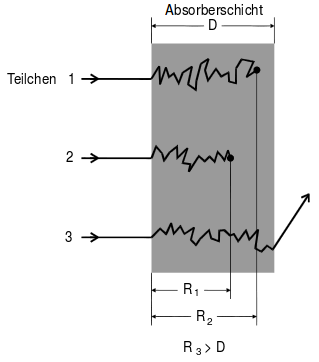
\includegraphics[width=0.4\textwidth]{Bilder/reichweite.png}
	\caption{Veranschaulichung der Reichweitenerhöhung der $\beta^-$-Strahlung in Materie. \cite{skript}}
	\label{fig:bahnen}
\end{figure}
Weitere, hier nicht weiter betrachtete Einflüsse der Strahlung durch die Materie ist an das magnetische Moment der Elektronen geknüpft.

\item{\emph{Inelastische Streuung an dem Atomkern des Absorbermaterials}}

Bewegen sich geladene Teilchen im Coulomb-Feld von entgegengesetzt geladenen Teilchen, so werden sie beschleunigt, 
wobei Energie in Form von Strahlung abgegeben werden muss.
Dies wird als inelastische Streuung an Atomkernen bezeichnet.
%Diese Strahlung ist für die Abbremsung verantwortlich und es gilt
%\begin{equation}
% 	\sigma_\text{Br}=\alpha r_\text{e}^2 z^2
% \end{equation} 
%mit der Sommerfeldschen Feinstruktur $\alpha$.
%Aus dieser Formel des Wirkungsquerschnitt folgt, dass die Bremsstrahlung vorzugsweise bei schweren Absorberatomen stattfindet.
%Unter der Berücksichtigung aller Ablenkungswinkel ist die mittlere Abbremsungsenergie $E_\text{Br}$ eines mit der Energie $E_\beta^-$ einfallenden Strahles etwa $E_\text{Br} = 7\cdot10^{-7}zE_\beta^-$.
%Diese Formel ist eine gültige Näherung für die meisten gängigen $\beta^-$-Strahler.

\item{\emph{Inelastische Streuung an den Elektronen des Absorbermaterials}}

Die inelastische Streuung an Elektronen führt zur Anregung oder zur Ionisierung von Absorberatomen.
Wegen der hohen kinetischen Energie der Strahlung ist $\beta^-$-Strahlung imstande, dies mehrfach auszuführen.
Bei geringer Energie, beispielsweise $E\approx\SI{150}{\kilo\electronvolt}$ bei Aluminium, ist aber damit zu rechnen, 
dass die $\beta^-$-Strahlung bereits ab einer Dicke von $\SI{150}{\micro\meter}$ vollständig abgebremst wird.
\end{itemize}


\begin{figure}[hbp]
	\centering
	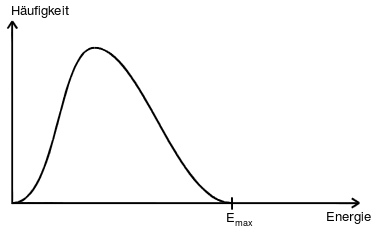
\includegraphics[width=0.5\textwidth]{Bilder/beta.png}
	\caption{Verteilung der kinetischen Energie von \texorpdfstring{$\beta$}{Beta}-Teilchen.\cite{skript}}
	\label{fig:energieElektron}
\end{figure}

\subsection{Messmethodik bei \texorpdfstring{$\beta^-$}{Beta}-Strahlung}
Obwohl die Gleichung \eqref{eq:Absorptionsgesetz} nicht im Allgemeinen für die $\beta^-$-Strahlung gilt, ist sie für geringe Blendendicken eine brauchbare Näherung.
Bei der Benutzung von Amplituden-sensitiven Messgeräten ergibt sich, dass ab einer Mindestschichtdicke eine von der Dicke unabhängigen Intensität gemessen werden kann, die auf die Bremsstrahlung zurückzuführen ist und wesentlich besser Materie durchdringt.
\begin{figure}[ht]
	\centering
	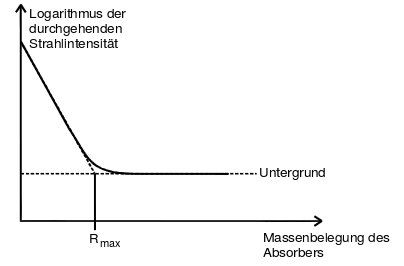
\includegraphics[width=0.5\textwidth]{Bilder/absorption.png}
	\caption{Strahlungsintensität in Abhängigkeit von der Massenbelegung $R$ und Bestimmung der maximalen Reichweite.\cite{skript}}
	\label{fig:messkurve}
\end{figure}
In Abbildung \ref{fig:messkurve} ist die messbare Intensität gegen die Massenbelegung $R$ -- als Maß der Dicke mit $R=\rho D$ -- erkennbar.
Mithilfe einer solchen Kurve kann die Reichweite von $\beta^-$-Strahlung bestimmt und damit die Energie abgeschätzt werden.
Es gilt empirisch
\begin{equation}
	E_\text{max}=1.92\sqrt{R_\text{max}^2+0,22R_\text{max}}\;[\si{\mega\electronvolt}]
\label{eq:e_max}
\end{equation}
